\hypertarget{ux7ec4ux7ec7ux591aux5143ux5316}{%
\subsubsection{组织多元化}\label{ux7ec4ux7ec7ux591aux5143ux5316}}

问题:什么是贡献的组织多元化?

\hypertarget{ux63cfux8ff0}{%
\paragraph{描述}\label{ux63cfux8ff0}}

组织多元化表示一个项目有多少组织参与,以及组织之间不同的参与程度。

\hypertarget{ux76eeux6807}{%
\paragraph{目标}\label{ux76eeux6807}}

\begin{itemize}
\tightlist
\item
  获取为项目做出贡献的组织列表。
\item
  查看各组织在特定时间内的贡献百分比。
\item
  查看组织结构在特定时间内的变化。
\item
  获取各组织相关的人员列表。
\end{itemize}

\hypertarget{ux5b9eux73b0}{%
\paragraph{实现}\label{ux5b9eux73b0}}

\begin{itemize}
\tightlist
\item
  从发生贡献的数据源收集数据。
\item
  确定贡献者的从属关系,对其从属组织作出准确评估。
\item
  关联贡献相关信息,并将其匹配至适当组织。
\item
  根据项目需求,您可能需要考虑:如何处理多个电子邮件地址、随时间变化的从属关系,承包商与员工的关系等问题。
\end{itemize}

\hypertarget{ux63d0ux4f9bux6307ux6807ux7684ux5de5ux5177}{%
\subparagraph{提供指标的工具}\label{ux63d0ux4f9bux6307ux6807ux7684ux5de5ux5177}}

\begin{itemize}
\item
  \href{https://chaoss.github.io/grimoirelab}{GrimoireLab}
  支持组织多元化指标,开箱即用。
  \href{https://github.com/chaoss/grimoirelab-sortinghat}{GrimoireLab
  SortingHat} 管理身份信息。
  \href{https://github.com/chaoss/grimoirelab-hatstall}{GrimoireLab
  Hatstall} 用户界面可以修正人员的组织从属关系,甚至记录从属关系的变化。

  \begin{itemize}
  \item
    查看
    \href{https://chaoss.biterg.io/app/kibana\#/dashboard/Community-Structure-by-Organization}{Bitergia
    Analytics 的 CHAOSS 实例}示例可视化效果。
  \item
    从
    \href{https://chaoss.github.io/grimoirelab-sigils/panels/community-structure-by-organization/}{GrimoireLab
    Sigils 面板集合}下载并导入包含此指标可视化效果示例的现成仪表板。
  \item
    按照说明向任意 GrimoreLab Kibiter 仪表板添加一个示例可视化效果:

    \begin{itemize}
    \tightlist
    \item
      新建一个饼状图

      \begin{itemize}
      \tightlist
      \item
        选择 \texttt{all\_onion} 索引
      \item
        指标切片大小:\texttt{Sum} 聚合,\texttt{contributions}
        字段,\texttt{Contributions} 自定义标签
      \item
        桶拆分切片:\texttt{Terms} 聚合,\texttt{author\_or\_name}
        字段,\texttt{metric:\ Contributions}
        排序依据,\texttt{Descending} 排列,\texttt{500}
        大小,\texttt{Organization} 自定义标签
      \end{itemize}
    \item
      屏幕截图示例
    \end{itemize}

    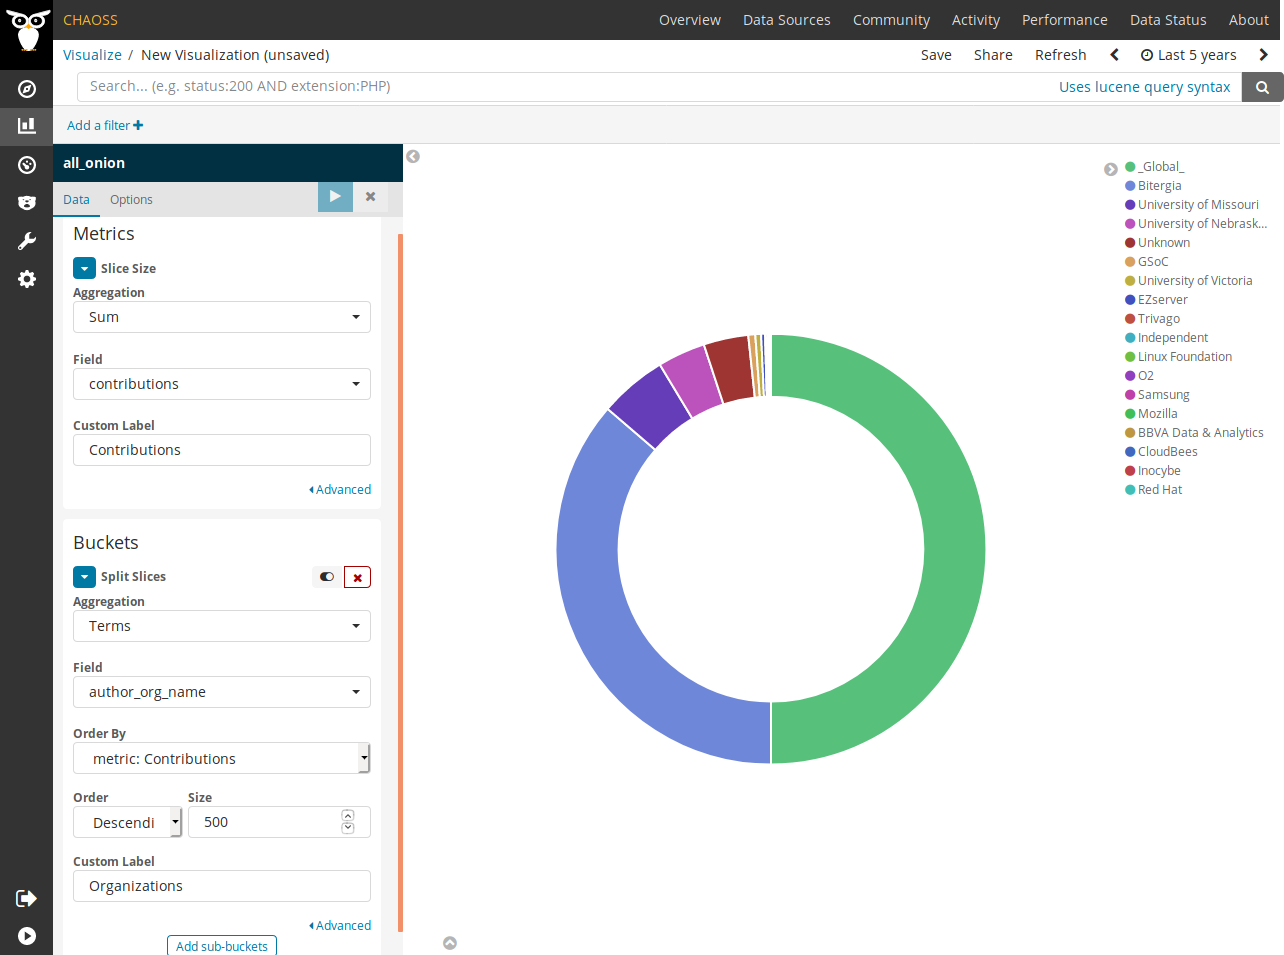
\includegraphics{images/organizational-diversity_piechart.png}
  \end{itemize}
\item
  \href{https://lfanalytics.io}{LF Analytics}
  在主视图中为提交、提交的问题和通信渠道(目前支持 Slack 和
  groups.io)提供组织多元化指标。
\end{itemize}

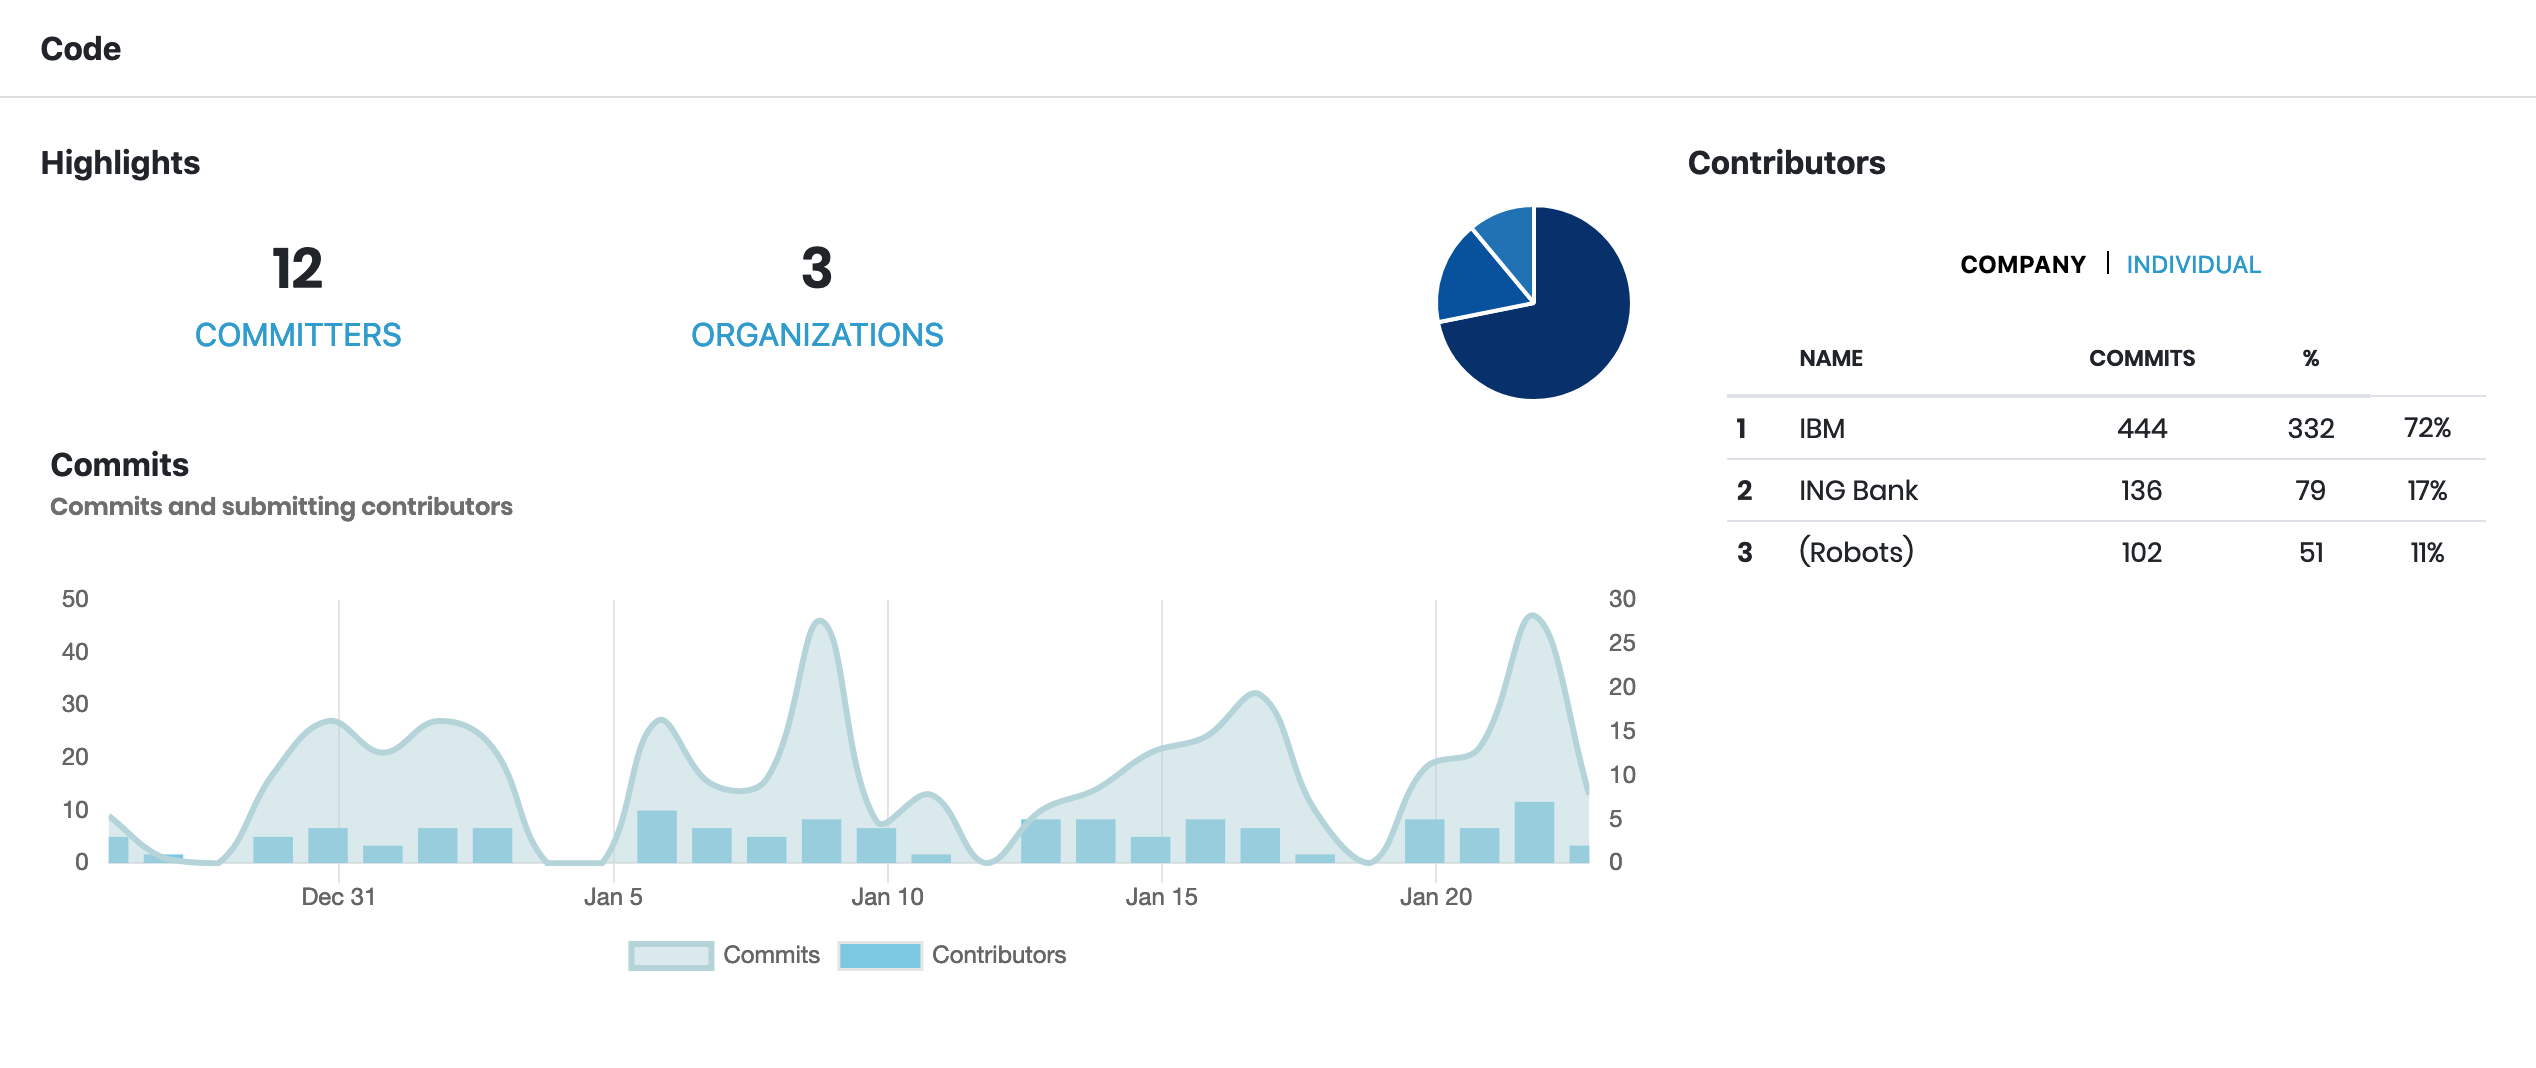
\includegraphics{images/organizational-diversity_lfanalytics-orgdiversity.png}

\hypertarget{ux6570ux636eux6536ux96c6ux7b56ux7565}{%
\subparagraph{数据收集策略}\label{ux6570ux636eux6536ux96c6ux7b56ux7565}}

\textbf{定性}

\begin{itemize}
\tightlist
\item
  组织在项目或生态系统中的足迹
\item
  组织在项目或生态系统中的影响
\item
  治理结构中的从属多元化。
\end{itemize}

\textbf{定量}

\begin{itemize}
\tightlist
\item
  每个组织的commits百分比
\item
  每个组织的merges/reviews百分比
\item
  每个组织的任意种类的贡献者百分比
\item
  每个组织贡献的代码行数百分比
\item
  每个组织提出的问题(issues)百分比
\item
  \href{https://github.com/chaoss/metrics/blob/master/activity-metrics/contributing-organizations.md}{贡献组织}
  - 贡献组织的数量是多少?
\item
  \href{https://github.com/chaoss/metrics/blob/master/activity-metrics/new-contributing-organizations.md}{新的贡献组织}
  - 新的贡献组织的数量是多少?
\item
  新贡献者组织 - 随着时间推移,对项目作出贡献的新组织。
\item
  贡献组织的数量 - 在一段时间内参与项目的组织数量。
\item
  大象系数 - 如果 50\%
  的社区成员受雇于同一家公司,那就形成了房间里的大象。 公式:员工完成
  50\% 提交次数的最小公司数量
\item
  \href{https://github.com/chaoss/metrics/blob/master/activity-metrics/contributor-diversity.md}{从属多元化}
  - 单个公司的贡献者在所有贡献者中的比例。 又称:来自不同公司的维护者。
  贡献者从属多元化。
\item
  在具有代码所有权概念的项目中,从属于每个组织的代码所有者的百分比,按其拥有的代码的重要性/大小/LoC
  和共同所有者的数量进行权衡。
\end{itemize}

\hypertarget{ux53c2ux8003ux8d44ux6599}{%
\paragraph{参考资料}\label{ux53c2ux8003ux8d44ux6599}}

\begin{itemize}
\tightlist
\item
  潜在实现和参考资料:

  \begin{itemize}
  \tightlist
  \item
    \href{https://bitergia.gitlab.io/panel-collections/open_source_program_office/organizational-diversity.html}{https://bitergia.gitlab.io/panel-collections/open\_source\_program\_office/organizational-diversity.html}
  \item
    \href{https://katacontainers.biterg.io}{Kata Containers
    仪表板条目页面}(底部)
  \item
    \href{https://github.com/chaoss/augur}{Augur}
  \end{itemize}
\end{itemize}
